\documentclass[12pt]{article}
\usepackage{amsmath}
\usepackage{graphicx}
\usepackage{booktabs}
\usepackage{lscape}
\usepackage[spanish,es-tabla]{babel}
\usepackage{adjustbox}
\usepackage{algorithm} 
\usepackage{algorithmic} 
\usepackage{hyperref} 

\begin {document}
\section{Modelos escalares y extensiones}
\subsection{Geometría de Riemann}
La geometría de Riemann es necesaria para entender las bases matemáticas que permiten definir los subespacios de características, los cuales son fundamentales a la hora de modelizar enfermedades. Para ello, es necesario explicar algunos conceptos clave. \\

En primer lugar, esta geometría se basa en el concepto de variedades. Son espacios en los cuales cada punto tiene una estructura suave y diferenciable similar al espacio euclidiano. Al haber zonas de la variedad conectadas con espacios lineales, se pueden realizar cálculos diferenciables localmente. Además, si a una variedad suave \textit{M} se le equipa con una colección de productos internos $g_{\textbf{M}}=(g_{\textbf{p}})_{\textbf{p}\in \textbf{M}}$, llamados métrica en la variedad y asociados al espacio tangente $\textbf{T}_{\textbf{p}}\textbf{M}$, se le llama variedad de Riemann. Este concepto introduce la noción de distancias en la estructura diferenciable de la variedad.\\

Por otra parte están las geodésicas, que son curvas que representan la trayectoria mas corta entre dos puntos en una variedad de Riemann. Son análogas a las lineas rectas en la geometría euclidiana. En el mapeo exponencial, se asocia un vector tangente a un punto con otro punto alcanzado por una geodésica a lo largo de la dirección del vector. Esto se representa con la siguiente función $\textbf{v}\in\textbf{T}_{\textbf{p}}\rightarrow Exp_{\textbf{p}}(\textbf{v})=Exp_{\textbf{p},t}(\textbf{v})(t+1)$.\\

Por último, para comparar cálculos en espacios tangentes a lo largo de una geodésica, es muy importante entender el \textbf{transporte paralelo}. Teniendo una curva suave $\gamma$ y dado un vector $\textbf{w}_{0}$ en el espacio tangente $\textbf{T}_{\gamma(t_{0})\textbf{M}}$, existe un único campo vectorial paralelo a lo largo de la curva tal que $\textbf{w}(t_{0})=\textbf{w}_{0}$.

\subsection{Modelo de efectos mixtos}
Los modelos de efectos mixtos son una herramienta que permite formular la trayectoria de la progresión de una enfermedad tanto de manera global como individual, algo que no se puede hacer con la geometría de Riemann. Esto es posible combinando dos tipos efectos:
\begin{itemize}
	\item Efectos globales o fijos: describen a la población en su conjunto. No son aleatorios.
	\item Efectos individuales o aleatorios: representan las variaciones especificas de cada observación. Son aleatorios.
\end{itemize}

A partir de los modelos de regresión clásicos, surgen dos métodos para el modelado de efectos mixtos, en función de su complejidad a la hora de capturar las interacciones entre variables de entrada y salida.


\begin{description}
	\item {\textbf{Modelos Lineales de Efectos Mixtos (LME)}}

Este modelo añade un grado de libertad más al modelo clásico de regresión lineal para capturar las variaciones especificas de cada sujeto, representándose de la siguiente manera:\\
\begin{center}
	$\textbf{y}_{i}=\textbf{x}_{i}\alpha+\textbf{z}_{i}\beta_{i}+\epsilon_{i}$
\end{center}
donde $\textbf{y}_{i}$ son la variables de resultado de la i-ésima observación, $\textbf{x}_{i}$ y $\textbf{z}_{i}$ son las entradas, los efectos fijos son $\alpha$ y los aleatorios de cada observación se corresponden con $\beta_{i}$.

	\item{\textbf{Modelos No Lineales de Efectos Mixtos (NLMEM)}}
	
Este modelo captura interacciones complejas entre las entradas y la salida. Su funcionamiento se representa con la siguiente ecuación:
\begin{center}
	$\textbf{y}_{i}=g(\textbf{x}_{i},\textbf{z}_{i})+\epsilon_{i}$
\end{center}
siendo \textit{g} una función no lineal de las variables de entrada.
\end{description}

Para describir la evolución de los datos longitudinales en el caso de fenómenos biológicos, se utiliza el modelo de pendiente aleatoria e intersección aleatoria. Describe la trayectoria de cada individuo en cada visita como una variación de pendiente e intersección con respecto a la trayectoria global y se representa con la siguiente función:
\begin{center}
	$\textbf{y}_{ij}=(\alpha^{1}+\beta_{i}^{1})t_{ij}+(\alpha^{2}+\beta_{i}^{2})+\epsilon_{ij}$
\end{center}
donde los efectos fijos de la trayectoria promedio son $\alpha^{1}$ (pendiente) y $\alpha^{2}$ (intersección) y los efectos aleatorios de cada sujeto se representan con $\beta_{i}^{1}$ (pendiente) y $\beta_{i}^{2}$ (intersección).\\

Este modelo se utiliza en casos en los que los eventos de los pacientes están alineados temporalmente. Por ello, para casos como el de la progresión de una enfermedad es necesario realizar una reparametrización del tiempo ajustando las observaciones individuales con un desplazamiento temporal ($t \rightarrow t-\tau_{i}$).

\subsection{Modelo de Progresión de la Enfermedad (DPM)}
En este apartado, se presenta un modelo de efectos mixtos con el cual se pretende definir la progresión general de la enfermedad así como la trayectoria especifica de cada individuo. Esto se consigue mediante el estudio de las medidas tomadas durante las visitas sucesivas de cada uno de los pacientes.\\

Para ello, cada observación tomada es considerada como parte de una variedad de Riemann y la progresión general de la enfermedad se representa con una geodésica (trayectoria promedio $\tau_{0}$). Además, las trayectorias individuales son modeladas como desviaciones espaciotemporales de la curva promedio en términos de dirección y velocidad. Teniendo la dirección definida en el desplazamiento espacial ($w_{i}$), la trayectoria individual se representaría con la siguiente función:
\begin{center}
	$\eta^{\textbf{w}_{i}}(t):=\exp_{\gamma_0(t)} (P_{\gamma_0,t_0,t}(\textbf{w}_i)))$
\end{center}
Mientras que la progresión temporal individual ($\eta^{\textbf{w}^{i}}(t)$) se ajusta con la siguiente reparametrización temporal:
\begin{center}
	$\psi_i:t \rightarrow \alpha_i(t - \tau_i - t_0) + t_0$
\end{center}
siendo $\alpha_i$ la aceleración, la cual indica una progresión mas rápida cuando es mayor que 1; y $\tau_{i}$ el desplazamiento temporal el cual indica una progresión más tardía cuando es menor que 0.\\

Las mediciones de cada individuo \textit{i} en el tiempo \textit{j} se definen como:
\begin{center}
	$\textbf{y}_{ij}=\eta^{\textbf{w}_{i}}(\psi_{i}(t_{ij}))+\epsilon_{ij}$
\end{center}

Estadísticamente, se puede comparar con un modelo de efectos mixtos donde la geodésica fija dentro de la configuración Riemannieana que modela la trayectoria promedio representarían los efectos fijos. Los efectos aleatorios serían las curvas individuales que se derivan de la geodésica mediante los parámetros de cada sujeto.\\

Además, es necesario asegurar las condiciones de identificabilidad del modelo. Cuando haya variabilidad espaciotemporal, se utiliza el método Householder para que el producto interno entre cada columna de la matriz A y $v_{0}$ debe sea cero y así garantizar que $\textit{w}_{i}$ sea ortogonal a la velocidad $v_{0}$.\\

A parte, en el modelo utilizado, la trayectoria general es percibida como un conjunto de trayectorias individuales en diferentes direcciones calculadas juntando la velocidad con unos ajustes concretos para cada observación \textit{j}.\\

\begin{table}[h]
	\begin{adjustbox}{width=\textwidth}
		\begin{tabular}{|l||l|}
			\toprule
			GRÁFICAS & FUNCIONES\\
			\hline
			\multicolumn{2}{ |l| }{(a) Lineas rectas paralelas} \\
			\hline
			\raisebox{-0.6\height}{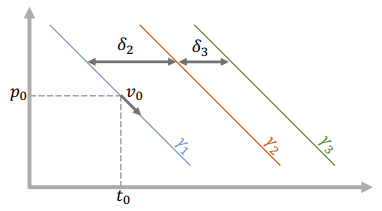
\includegraphics[width=3cm]{im1}} & \begin{tabular}{@{}l@{}} $g_p^k(u, v) = uv$ \\
				$\gamma_k(t) = p_0 + (t - t_0 - \delta_k)v_0$ \\
				$\eta_{k}^{\textbf{w}_{i}}(\psi_{i}(t_{ij})) = w_{ik} + p_{0} + (\alpha_{i}(t_{ij}-t_{0}-\tau_{i})+\delta_{k})v_{0}$ \end{tabular}\\
			\hline
			\multicolumn{2}{ |l| }{(b) Lineas rectas} \\
			\hline
			\raisebox{-0.5\height}{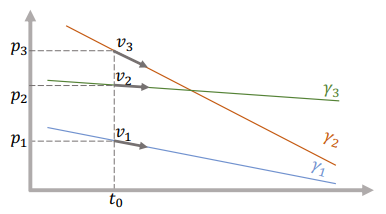
\includegraphics[width=3cm]{im2}} & \begin{tabular}{@{}l@{}} $g_p^k(u, v) = uv$ \\
				$\gamma_k(t) = p_k + (t - t_0)v_k$ \\
				$\eta_{k}^{\textbf{w}_{i}}(\psi_{i}(t_{ij})) = w_{ik} + p_{k} + \alpha_i(t_{ij}-t_{0}-\tau_{i})v_{k}$\end{tabular} \\
			\hline
			\multicolumn{2}{ |l| }{(c) Formas logísticas paralelas} \\
			\hline
			\raisebox{-0.6\height}{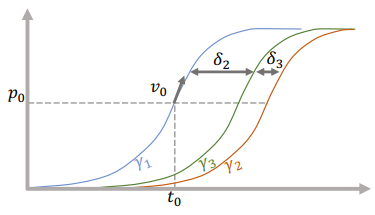
\includegraphics[width=3cm]{im3}} & \begin{tabular}{@{}l@{}} $g_p^k(u, v) = \frac{uv}{p^{2}(1-p)^{2}}$ \\
				$\gamma_k(t) = (1+(\frac{1}{p_{0}}-1)E(t))^{-1}$ \\
				$\eta_{k}^wi(\psi_i(t_{ij})) = (1+(\frac{1}{p_{0}}-1)\exp (\frac{-v_{0}(\alpha_{i}(t-\tau_{i}-t_{0})+\delta_{k})}{p_{0}(1-p_{0})}-\frac{w_{ik}(1+gE(t_{0}))^{2}}{gE(t_{0})}))^{-1}$\end{tabular} \\
			\hline
			\multicolumn{2}{ |l| }{(d) Formas logísticas} \\
			\hline()
			\raisebox{-0.5\height}{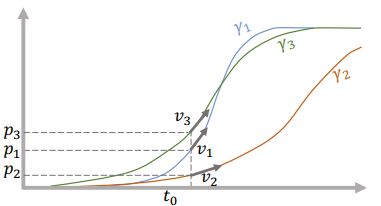
\includegraphics[width=3cm]{im4}} & \begin{tabular}{@{}l@{}} 
				$g_p^k(u, v) = \frac{uv}{p^{2}(1-p)^{2}}$\\
				$\gamma_k(t) = (1+(\frac{1}{p_{k}}-1)\exp(-\frac{v_{k}}{p_{k}(1-p_{k})}(t-t_{0})))^{-1}$ \\
				$\eta_{k}^wi(\psi_i(t_{ij})) = (1+(\frac{1}{p_{k}}-1)\exp (-\frac{w_{ik}+v_{k}\alpha_{i}(t_{ij}-\tau_{i}-t_{0})}{p_{k}(1-p_{k})}))^{-1}$\end{tabular} \\
			\hline
			\multicolumn{2}{ |l| }{(e) Decaimientos exponenciales paralelos} \\
			\hline
			\raisebox{-0.5\height}{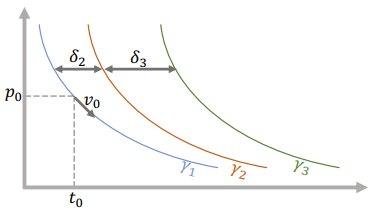
\includegraphics[width=3cm]{im5}} & \begin{tabular}{@{}l@{}} 
				$g_p^k(u, v) = \frac{uv}{p^{2}}$ \\
				$\gamma_k(t) = p_{0}\exp(-\frac{v_{0}}{p_{0}}(t-t_{0}+\delta_{k}))$ \\
				$\eta_{k}^wi(\psi_i(t_{ij})) = p_{0}\exp(-\frac{w_{i}k}{p_{0}}-\frac{v_{0}}{p_{0}}(\alpha_{i}(t_{ij}-t_{0}-\tau_{i})+\delta_{k}))$\end{tabular} \\
			\hline
			\multicolumn{2}{ |l| }{(f) Decaimientos exponenciales} \\
			\hline
			\raisebox{-0.5\height}{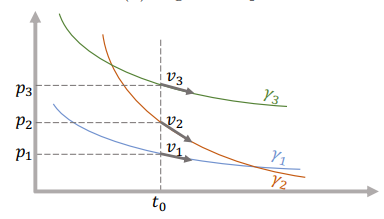
\includegraphics[width=3cm]{im6}} & \begin{tabular}{@{}l@{}} 
				$g_p^k(u, v) = \frac{uv}{p^{2}}$ \\
				$\gamma_k(t) = p_{k}\exp(-\frac{v_{k}}{p_{k}}(t-t_{0}))$ \\
				$\eta_{k}^wi(\psi_i(t_{ij})) = p_{k}\exp(-\frac{w_{ik}}{p_{k}}-\frac{v_{k}\alpha_{i}}{p_{k}}(t_{ij}-t_{0}-\tau_{i}))$\end{tabular} \\
			\bottomrule
		\end{tabular}
	\end{adjustbox}
	\caption{Instanciaciones del modelo genérico}
	\label{tab:tabla1}
\end{table}


\subsection{Modelo de Progresión de la Enfermedad (DPM)}
En la tabla \ref{tab:tabla1} vemos seis distintas formas de instanciar el modelo genérico: 
\begin{enumerate}
	\item \textbf{Lineas rectas paralelas.} Cada geodésica \textit{k} realiza una traslación horizontal de valor $\delta_{k}$ y alcanzan el valor $p_{0}$ con velocidad $v_{0}$ y tiempo $t_{0}+\delta_{k}$.
	\item\textbf{ Lineas rectas.} Representan geodésicas que alcanzan el valor $p_{k}$ con velocidad $v_{k}$ en el tiempo $t_{0}$.
	\item \textbf{Formas logísticas paralelas.} \textit{K} dimensiones representadas por curvas logísticas con valores entre 0 y 1, retrasadas por un tiempo $\delta_{k}$ y que alcanzan $p_{0}$ en el tiempo $t_{0}$ con velocidad $v_{0}$.
	\item \textbf{Formas logísticas.} Cada coordenada es independiente, alcanzando el valor $p_{k}$ en el tiempo $t_{0}$ con velocidad $v_{k}$.
	\item \textbf{Decaimientos exponenciales paralelos.} Geodésicas como curvas exponenciales decrecientes que van desde $-\infty$ finalizando en 0, trasladadas las curvas \textit{k} un tiempo $\delta_{k}$.Alcanzan $p_{0}$ con $v_{0}$ en t igual a $t_{0}$.
	\item \textbf{Decaimientos exponenciales.} Alcanzan el valor $p_{k}$ en el tiempo $t_{0}$ con velocidad $v_{k}$.
\end{enumerate}

En cada uno de ellos se refleja la función de $g_{p}^{k}$, la ecuación de la geodésica de una dimensión $\gamma_{k}$  y la coordenada k de la trayectoria individual $\eta_{k}^{\textbf{w}_{i}}(\psi_{i}(t_{ij}))$. \\

Para cambiar estos seis modelos se pueden realizar algunas variaciones disponibles en softwares como Leaspy. Entre ellas encontramos las siguientes:
\begin{itemize}
	\item Parametrización de formas distintas aplicables a los distintos modelos: valor $p_{0}$ alcanzado con velocidad $v_{0}$ en distintos momento, o valores $p_{1}$ a $p_{n}$ alcanzados por un solo momento.
	\item Modelos univariantes en los que establecer $\textbf{w}_{i}=(\textbf{w}_{i1})=0$ para poder usar los modelos mencionados.
	\item Número de fuentes ($\textit{N}_{S}$) las cuales definen el subespacio de posibles direcciones para el desplazamiento espacial. El valor ideal de esta variable es el mínimo que consigue saturar el ruido.
\end{itemize}

Una vez conocemos las distintas opciones de modelos posibles, es necesario saber como reconocer cual es el que mejor cumple las necesidades. Entre los factores a considerar están el proceso biológico en cuestión, el número de sujetos del estudio y el numero de puntos temporales disponibles en los datos. Tener en cuenta todo esto es necesario para escoger un modelo que represente con precisión la población estudiada y su evolución.



\end{document}